% Copyright (c) 2021 Tobias Briones. All rights reserved.
%
% SPDX-License-Identifier: CC-BY-4.0
%
% This file is part of Course Project at UNAH-MM700: Agricultural Soil Sampling
% for Data Analysis.
%
% This source code is licensed under the Creative Commons Attribution 4.0
% International License found in the LICENSE-CC file in the root directory of
% this source tree or at https://spdx.org/licenses/CC-BY-4.0.html.

\documentclass{article}
\usepackage{annexes}

\title{Anexos de Investigación: Modelo de Muestreo Virtual de Suelos Agrícolas en Honduras para Analítica en Base al Muestreo Aleatorio Simple y Estratificado}
\author{Tobias Briones \bigbreak tobias.briones@unah.hn}
\date{Diciembre 2021}

\begin{document}

\makeatletter
    \begin{titlepage}
        \begin{center}
            
\includegraphics[width=0.3\linewidth]{ref/logo-unah.png}\\[4ex]
            {\huge \bfseries \@title 
            \vspace{1cm}}\\[2ex]
            {\LARGE \@author}\\[50ex] 
            
            {\large
            Proyecto de Seminario de Investigación Presentado a la\\
            Universidad Nacional Autónoma de Honduras de la Carrera de\\
            Licenciatura en Matemática
            }\\[2ex]
            
            {\large \@date}
        \end{center}
    \end{titlepage}
\makeatother
\thispagestyle{empty}
\newpage

\section{Anexos}

\subsection{Introducción}

\begin{lstlisting}[language=Python, caption=Introducción al enunciados del problema]
from main import plot
from test import hn_example as hn

# ----------

hn_gis = hn.Gis()

hn_gis.parent_dir = './test'

# ----------

# SIG

hn_gdf = hn_gis.load()
hn_df = hn_gis.df()

hn_df

# ----------

# Muestreo fisico (generado aleatoriamente)

hard_sampling = hn.HardSampling.generate()

hard_sampling

# ----------

# SIG

plot(hn_gdf, 'Mapa de Suelo Agricola por Lotes', size=20)

# Mapa de Suelo Agricola por Estratos
hn_gdf.plot(figsize=(20, 20), column=hn.STRATUM_COL, legend=True)

# ----------

from test import main
import sampling

main = main.Main.new_instance('./test')
sampling = sampling.Sampling.from_main(main)
sim = sampling.new_sampling_simulator()

sampling.stratum_sampling_size(300)

sim.simulate(hn.Stratum.CP_72_2086)
\end{lstlisting}

\begin{figure}[H]
    \centering
    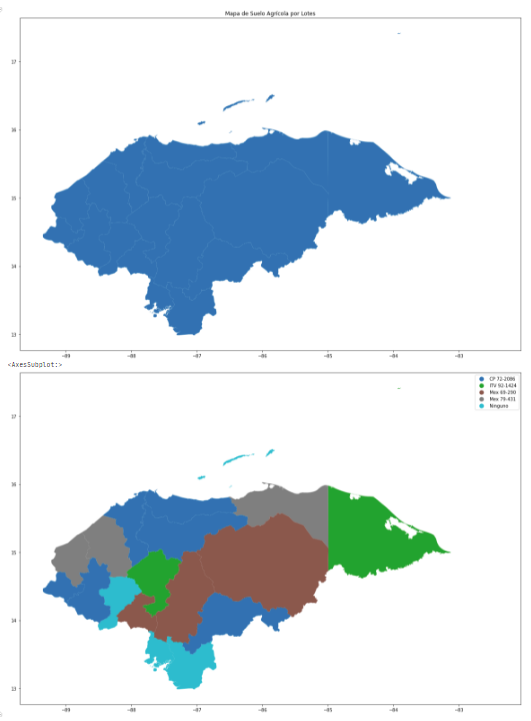
\includegraphics[width=0.5\paperwidth]{ref/intro-fig-1.png}
    \caption{Mapa del suelo agrícola}
    Fuente: Derivado de GADM data (version 3.6) \cite{gadm-2021}
\end{figure}

\begin{figure}[H]
    \centering
    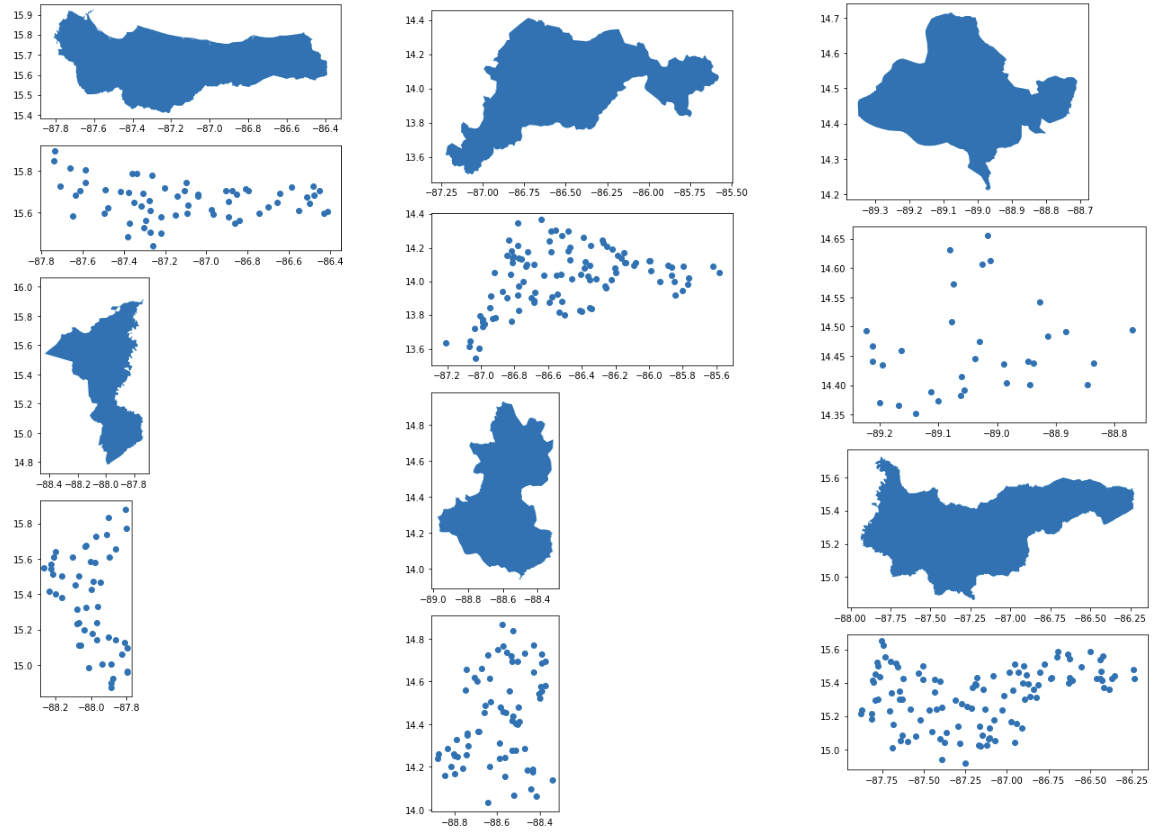
\includegraphics[width=0.3\paperwidth]{ref/intro-fig-2.png}
    \caption{Simulación de muestreo virtual para el estrato $CP \,\, 72-2086$}
    Fuente: Derivado de GADM data (version 3.6) \cite{gadm-2021}
\end{figure}

\subsection{Código fuente}

Se recomienda obtener una copia del código fuente desde el proyecto en GitHub dado en las recomendaciones. Sin embargo, se adjunta una copia ligera sin documentación a continuación.


\bigbreak

\begin{lstlisting}[language=Python, caption=test/main.py]
from . import hn_example as hn

DEF_STRATUM_COL = 'Estrato'

class Main:
    @staticmethod
    def new_instance(parent_dir='.'):
        gis = hn.Gis(parent_dir)
        df = hn.HardSampling.generate()

        gis.load()
        return Main(gis, df)

    def __init__(self, gis, df):
        self.__gis = gis  # Immutable
        self.__df = df  # Immutable

    def gis(self):
        return self.__gis

    def gdf(self):
        return self.__gis.gdf()

    def df(self):
        return self.__df

    def cols(self):
        return cols()

    def filter(self):
        valid_stratum = self.__df[DEF_STRATUM_COL] != hn.Stratum.NONE
        self.__df = self.__df[valid_stratum].reset_index(drop=True)


class ColumnConfig:
    def __init__(
        self,
        stratum='stratum',
        harvested_area='harvested_area',
        gis_area='area',
        gis_subset='subset'
    ):
        self.stratum = stratum
        self.harvested_area = harvested_area
        self.gis_area = gis_area
        self.gis_subset = gis_subset


def cols():
    return ColumnConfig(
        stratum=hn.STRATUM_COL,
        harvested_area=hn.HardSampling.HARVESTED_AREA_COL,
        gis_area=hn.Gis.AREA_COL,
        gis_subset=hn.Gis.DEPARTMENT_COL
    )
\end{lstlisting}




\bigbreak





\begin{lstlisting}[language=Python, caption=test/hn\_example.py]
import random
import functools
import numpy as np
import pandas as pd
import geopandas as gpd
from strenum import StrEnum

STRATUM_COL = 'Estrato'

class Stratum(StrEnum):
    NONE = 'Ninguno'
    CP_72_2086 = 'CP 72-2086'
    MEX_69_290 = 'Mex 69-290'
    MEX_79_431 = 'Mex 79-431'
    ITV_92_1424 = 'ITV 92-1424'


class Gis:
    FILE_NAME = '/data/gis/gadm36_HND_1.shp'
    DEPARTMENT_COL = 'NAME_1'
    AREA_COL = 'Area Departamento (HA)'

    def __init__(self, parent_dir='.'):
        self.parent_dir = parent_dir
        self.__gdf = gpd.GeoDataFrame()

    def df(self):
        data = self.__gdf.drop(columns='geometry')
        return pd.DataFrame(data)

    def gdf(self):
        return self.__gdf

    def load(self):
        df = Gis.get_df()
        gdf_data = gpd.read_file(self.parent_dir + Gis.FILE_NAME)
        self.__gdf = gpd.GeoDataFrame(df, geometry=gdf_data.geometry)
        return self.__gdf

    @staticmethod
    def get_df():
        departments = [
            'Atlantida',
            'Choluteca',
            'Colon',
            'Comayagua',
            'Copan',
            'Cortes',
            'El Paraiso',
            'Francisco Morazan',
            'Gracias a Dios',
            'Intibuca',
            'Islas de la Bahia',
            'La Paz',
            'Lempira',
            'Ocotepeque',
            'Olancho',
            'Santa Barbara',
            'Valle',
            'Yoro'
        ]

        strata = [
            Stratum.CP_72_2086,
            Stratum.NONE,
            Stratum.MEX_79_431,
            Stratum.ITV_92_1424,
            Stratum.MEX_79_431,
            Stratum.CP_72_2086,
            Stratum.CP_72_2086,
            Stratum.MEX_69_290,
            Stratum.ITV_92_1424,
            Stratum.NONE,
            Stratum.NONE,
            Stratum.MEX_69_290,
            Stratum.CP_72_2086,
            Stratum.CP_72_2086,
            Stratum.MEX_69_290,
            Stratum.MEX_79_431,
            Stratum.NONE,
            Stratum.CP_72_2086
        ]

        areas_km2 = [
            4227,
            4397,
            8875,
            5120,
            3239,
            3911,
            7383,
            8619,
            15876,
            3126,
            229,
            2534,
            4285,
            1636,
            24038,
            5013,
            1618,
            7787
        ]

        areas_ha = list(map(lambda a: a * 100, areas_km2))

        return pd.DataFrame({
            Gis.DEPARTMENT_COL: departments,
            STRATUM_COL: strata,
            Gis.AREA_COL: areas_ha
        })


class HardSampling:
    YIELD_COL = 'TA/HA Real'
    HARVESTED_AREA_COL = 'Area Cosechada (HA)'
    POPULATION_SIZE = 100_000

    @staticmethod
    def generate():
        variety_data = pd.DataFrame(
            random.choices(
                list(Stratum),
                k=HardSampling.POPULATION_SIZE
            ),
            columns=[STRATUM_COL]
        )
        area_data = pd.DataFrame(
            np.random.randint(
                0.1,
                50_000,
                (HardSampling.POPULATION_SIZE, 1)
            ) / 10,
            columns=[HardSampling.HARVESTED_AREA_COL]
        )
        yield_data = pd.DataFrame(
            np.random.randint(0, 100, (HardSampling.POPULATION_SIZE, 1)) / 10,
            columns=[HardSampling.YIELD_COL]
        )
        data = [variety_data, area_data, yield_data]
        return functools.reduce(
            lambda left, right: pd.merge(
                left,
                right,
                left_index=True,
                right_index=True
            ),
            data
        )
\end{lstlisting}





\bigbreak




\begin{lstlisting}[language=Python, caption=sampling.py]
import random
import numpy as np
import pandas as pd
import geopandas as gpd
import plotly.express as px
from IPython.core.display import display

DEF_STRATUM_SAMPLING_SIZE = 1_000

class Sampling:
    @staticmethod
    def from_main(main):
        return Sampling(main.gis(), main.df(), main.cols())

    def __init__(self, gis, df, cols):
        self.__gis = gis  # Immutable
        self.__df = df  # Immutable
        self.__cols = cols  # Immutable
        self.__n = DEF_STRATUM_SAMPLING_SIZE
        self.__stratum_filter = StratumFilter(df, cols)

    def stratum_sampling_size(self, value):
        self.__n = value

    def stratum_filter(self):
        return self.__stratum_filter

    def run(self):
        sampling = pd.DataFrame(self.__df, copy=True)

        sampling = self.__stratum_filter.filter_df(sampling)
        sampling = self.__stratified_random_sampling(sampling)
        sampling = sampling.reset_index(drop=True)
        return Result(
            sampling,
            self.__stratum_filter
        )

    def new_sampling_simulator(self):
        return SamplingSimulator(self.__n, self.__cols, self.__gis)

    def __stratified_random_sampling(self, df):
        grouped = df.groupby(self.__cols.stratum)
        sampled_strata = []

        for name, group in grouped:
            stratum_df = group.reset_index(drop=True)
            sample = self.__random_sampling(stratum_df)
            sampled_strata.append(sample)
        return pd.concat(sampled_strata)

    def __random_sampling(self, stratum_df):
        h_n = stratum_df[stratum_df.columns[0]].count()
        units = random.sample(range(0, h_n - 1), self.__n)
        return stratum_df.filter(items=units, axis=0)


class Result:
    def __init__(
        self,
        sampling,
        stratum_filter
    ):
        self.__sampling = sampling
        self.__stratum_filter = stratum_filter

    def sampling(self):
        return self.__sampling

    def show_sampling(self):
        display(self.__sampling)

    def show_stratum_filter(self):
        self.__stratum_filter.plot_stratum_areas()
        display(self.__stratum_filter.result())


class StratumFilter:
    def __init__(self, df, cols):
        self.__df = df
        self.__cols = cols
        self.__area_threshold = 0
        self.__result = pd.DataFrame()

    def area_threshold(self, value):
        self.__area_threshold = value

    def result(self):
        return self.__result

    def filter_df(self, df):
        self.filter()
        strata = self.to_list()
        significant_stratum = df[self.__cols.stratum].isin(strata)
        return df[significant_stratum]

    def filter(self):
        areas = self.stratum_areas()
        curated = areas[
            areas[self.__cols.harvested_area] > self.__area_threshold
            ]
        self.__result = curated.reset_index(drop=True)
        return self.__result

    def to_list(self):
        return list(self.__result[self.__cols.stratum])

    def plot_stratum_areas(self):
        fig = px.bar(
            self.stratum_areas(),
            x=self.__cols.stratum,
            y=self.__cols.harvested_area
        )

        fig.show()

    def stratum_areas(self):
        grouped = self.__df.groupby(self.__cols.stratum)[
            self.__cols.harvested_area
        ]
        return grouped.sum().reset_index()


class SamplingSimulator:
    def __init__(self, h_n, cols, gis):  # Immutable
        self.__h_n = h_n
        self.__cols = cols
        self.__gis = gis

    def simulate(self, stratum):
        gdf = self.__gis.gdf()
        idx = self.__get_stratum_idx(stratum)

        for i, row in idx.iterrows():
            subset, subset_n = (row[self.__cols.gis_subset], int(row['n']))
            current_gdf = gdf[gdf[self.__cols.gis_subset] == subset]
            points = self.__random_points(subset_n, current_gdf)

            current_gdf.plot()
            points.plot()

    def __get_stratum_idx(self, stratum):
        df = self.__gis.df()
        sample_stratum = df[df[self.__cols.stratum] == stratum]
        total_area = sample_stratum[self.__cols.gis_area].squeeze().sum()
        sample_stratum.loc[:, 'weight'] = sample_stratum[
                                              self.__cols.gis_area
                                          ] / total_area
        sample_stratum.loc[:, 'n'] = sample_stratum['weight'] * self.__h_n

        return pd.DataFrame({
            self.__cols.gis_subset: sample_stratum[self.__cols.gis_subset],
            'n': sample_stratum['n']
        })

    @staticmethod
    def __random_points(n, gdf):
        x_min, y_min, x_max, y_max = gdf.total_bounds
        x = np.random.uniform(x_min, x_max, n)
        y = np.random.uniform(y_min, y_max, n)

        points = gpd.GeoSeries(gpd.points_from_xy(x, y))
        points = points[points.within(gdf.unary_union)]
        return points
\end{lstlisting}


\bigbreak


\end{document}
